\section{Traditional Distributed Computing Model}
\label{sec:traditional-distributed-computing}

Distributed computing systems are inherently distributed systems, which means
they share the fundamental characteristics and goals, defined by
\citeauthor{tannenbaum2017} \cite{tannenbaum2017} as resource sharing,
transparent distribution, openness, and scalability. Distributed computing
facilitate distributed system principles in order to group a set of resources
(possibly at a geographical distance) and provide tenants a single, coherent
view of these resources. In general distributed computing systems allow users to
share, manage the access to, and use compute, storage, and network resources.

In the following two sections we will look at two major distributed computing
concepts, Grid and Cloud computing.

\subsection{Grid Computing}

The Grid Computing model focuses on sharing widely distributed compute resources
in order provide problem-solving environments and enable collaboration for a set
of individuals or institutions, so-called virtual organizations. It provides
basic mechanisms, in the form of network protocols and interfaces. These
protocols and interfaces offer means of discovering, managing the access to, and
using remote resources. Because those resources are not subject to centralized
control, these protocols and interfaces have to be standardized and open to
enable interoperability \cite{foster2001grid}.

The hourglass model facilitated by the internet protocol stack can also be found
in the Grid computing architecture. While the base of the hourglass provides
various fundamental behaviors, the neck defines a small set of abstractions,
allowing a diverse set of high-level behaviors to be built on top. The four
layers of the Grid computing model are as follows:

\begin{figure}[H]
  \centering
  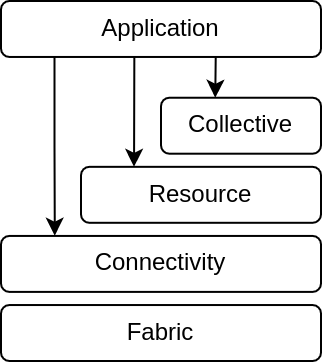
\includegraphics[width=0.3\linewidth]{resources/grid-architecture.drawio.png}
  \caption[The layered Grid architecture.]{
    The layered Grid architecture.\\
    Source: \citeauthor{foster2001grid} \cite{foster2001grid}
  }
  \label{fig:grid-architecture}
\end{figure}

\begin{description}
  \item[Fabric Layer]
    The Fabric layer provides the resources which are shared by Grid protocols
    and offers local, resource-specific operations that occur on specific
    resources as a result of sharing operations at higher levels. This should at
    least provide resource enquiry mechanisms, enabling the discovery of their
    structure, state and capabilities, and resource management mechanisms,
    providing control over them.
  \item[Connectivity]
    This layer specifies core communication and authentication protocols,
    enabling the exchange of data between Fabric layer resources and providing
    secure mechanisms for verifying the identity of users and resources.
    Communication usually requires transport, routing, and naming protocols.
  \item[Resource]
    On top of the Connectivity layer the Resource layer defines protocols
    providing secure negotiation, initiation, monitoring, control, accounting,
    and payment mechanisms for individual resources. It utilizes Fabric layer
    functions in order to access and control local resources. These protocols
    are focused on a single resource, implying that they ignore issues of global
    state and atomic actions across distributed collections.
  \item[Collective]
    While the Resource layer is concerned with the interactions of a single
    resource, the Collective layer focuses on the interaction of a collection of
    resources. Being the top and building on the neck (Connectivity and Resource
    layer) of the hourglass allows this layer to provide a wide variety of
    behaviors, such as discovering, co-allocation, scheduling, brokering,
    monitoring, and replication of resources.
  \item[Applications]
    The final layer of the Grid architecture is the collection of user
    applications. These applications implement specific business logics by
    utilizing resources and services of the previous layers.
\end{description}

\subsection{Cloud Computing}

Cloud Computing systems usually have a centralized control and facilitate both
open and proprietary protocols and interfaces in order to provide on-demand
self-service, broad network access, resource pooling, rapid elasticity, and
measured services. \citetitle{mell2011} \cite{mell2011} defines three distinct
service models of cloud computing:

\begin{description}
  \item[Infrastructure as a Service (IaaS)]
    In an IaaS service model the managed resources are fundamental computing
    resources. This includes -- physical or virtual -- machines, storage, and
    networks. The consumer does not manage or control the underlying
    infrastructure but can deploy and run arbitrary software, including
    operating systems, onto the provided infrastructure.

  \item[Platform as a Service (PaaS)]
    The PaaS service model adds another layer of abstraction on top of the IaaS
    service model. Consumers can deploy and run applications on a provided
    platform that supports a set of programming languages, libraries, services,
    and tools. So the managed resources in a PaaS service model are
    applications. The consumer does not manage or control the underlying
    infrastructure, and additionally has no control over the operating system.

  \item[Software as a Service (SaaS)]
    In this model the managed resources are applications. But in comparison to
    the PaaS model the consumer is not able to run arbitrary applications, but
    only a provider specific selection of applications. The customer does not
    manage or control the underlying infrastructure, operating system, or even
    the application.
\end{description}

These service models provide tenants with resources that applications run on and
services that support the development and deployment of these applications.

\subsection{Trust Model}

There are three roles that are present in the traditional distributed computing
model.

\begin{description}
  \item[Service Provider]
    In general a service provider is an entity or organizational unit that
    provides services to other entities or organizational units. In the
    distributed computing context service providers provide application owners
    and data owners with infrastructure resources and/or platform services.

  \item[Application Owner]
    Application owners manage applications that operate on data owned by the
    data owner. This does not imply that the application owner develops
    applications. Applications can be developed and provided by separate
    entities.

  \item[Data Owner]
    Data owners are in the possession of data that used, and/or manipulated by
    an application. They are concerned about the confidentiality of their data.
    If there are multiple data owners there may be mutual distrust between the
    data owners.
\end{description}

This trust model needs to be applied from the perspective of the data owners and
is tied to a set of data. For example, in a Grid environment, there are three
virtual organizations $A$, $B$, and $C$, all sharing resources and services.
Assuming that virtual organization $A$ owns a dataset $D$, but all of $A$'s
resources are currently occupied. Therefore, $A$ wants to use resources from
virtual organization $B$ in order to run an application on dataset $D$. In this
context, while all virtual organizations share resources, only $B$ takes on the
role of a service provider, because $A$ does not share resources used for this
specific context and $C$ is not involved at all. Because $A$ manages the
application and owns the dataset $D$, $A$ takes on the role of application owner
and data owner in this example.

Traditionally, the data owner trusts both the application owner and the service
provider. Therefore, both roles can be taken on by the same party.

\subsection{Architectural Overview}

\begin{figure}[H]
  \centering
  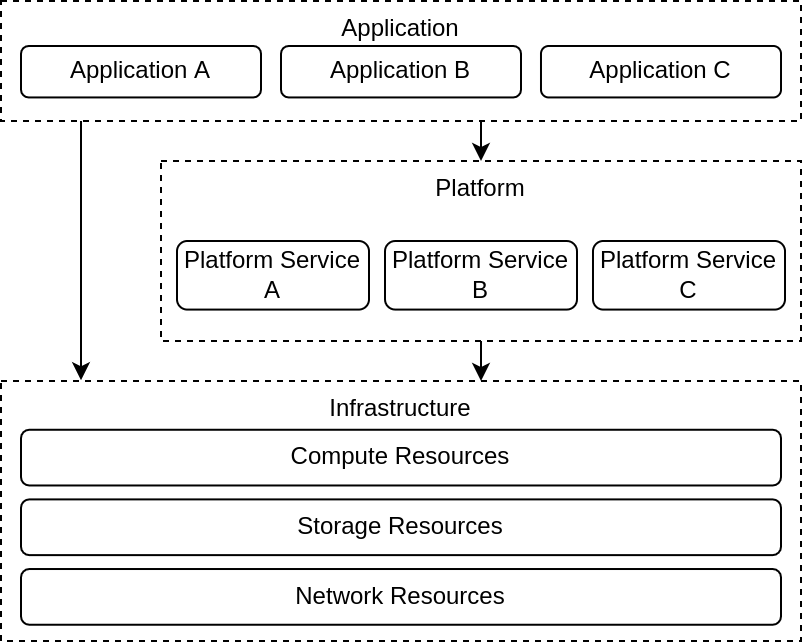
\includegraphics[width=0.7\linewidth]{resources/distributed-computing-overview.drawio.png}
  \caption{Layered model of a distributed computing system.}
\end{figure}

This section defines a generalized architecture of the distributed computing
model, which consists of three layers.

\begin{description}
  \item[Infrastructure]
    This layer provides fundamental resources, such as compute, network, and
    storage resources. This commonly includes physical or virtual machines
    (compute resource), layer two or three networks connecting machines (network
    resource), and network attached storage (storage resource).

    In the Cloud model this corresponds to the IaaS service model and in the
    Grid architecture it is represented by the Fabric layer.
  \item[Platform]
    The Platform layer sits between the Infrastructure and Application layer. It
    provides a set of services and tools that support application owners to run
    applications in a distributed computing environment and manage the
    underlying infrastructure resources required for the application to run. The
    platform layer abstract the complexity of the underlying infrastructure by
    providing services to manage, access, and utilize needed resources. These
    services are all operated and provided by the service provider.

    This layer matches the Cloud's PaaS and SaaS service model and is
    represented by the collection of the Resource, Connection, and Collective
    layer in the Grid architecture.
  \item[Application]
    The final layer is the collection of applications and services managed by
    application owners.
\end{description}

In the following figures components of the Infrastructure layer are marked in
blue, Platform layer in red, and Application layer in green.

\subsubsection{Infrastructure Layer}

\begin{figure}[H]
  \centering
  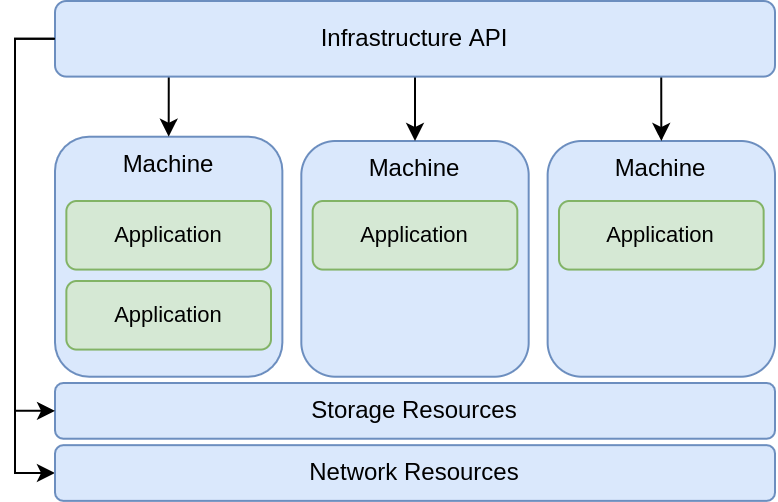
\includegraphics[width=0.7\linewidth]{resources/distributed-computing-infrastructure-example.drawio.png}
  \caption{Overview of the Infrastructure layer in the traditional distributed computing model.}
  \label{fig:traditional-infrastructure-overview}
\end{figure}

Typically, computing resources provided by the Infrastructure layer are in the
form of physical or virtual machines. These machines combine CPUs, memory, and
peripheral devices. On the other hand, storage and network resources can be
provided in various forms, such as block-level, file-level, and object-level
storage, and layer two and three networks. In order to keep this model abstract,
we will not make any assumptions about specifics of the storage and network
resources. This model will assume the presence of an application programming
interface (API), that can be used to implement a user interface. While various
kinds of user interfaces can be provided to tenants, such as websites, web
portals, terminal user interfaces (TUIs), graphical user interfaces (GUIs),
software development kits (SDKs), and libraries, these user interfaces typically
facilitate an API that exposes resource management actions.

As outlined before, there are two types of resources in the Infrastructure
layer: physical and virtual. Physical Infrastructure layer resources protection
is implemented by the service providers. For example by securing the physical
location of the hardware and utilizing application transparent encryption.
Virtual infrastructure is protected by the isolation that virtualization systems
provide. This requires a correctly configured and actively patched
virtualization system, as misconfiguration can lead to breaking the isolation
guarantees, and not patching virtualization systems allows attackers to exploit
vulnerabilities in those implementations. For example hypervisors are large
pieces of software that require complex configuration, and over the years
numerous vulnerabilities have been found in commonly used hypervisors
\cite{perezbotero2013hypervisorvulnerabilities,
  reuben2007surveyvirtualmachinesecurity}. These virtualization systems are
generally managed and controlled by the service provider. Therefore, protection
of infrastructure layer resources, regardless of whether the resources are
physical or virtual, is entrusted to the service provider.


\subsubsection{Platform Layer}

The platform layer offers various kinds of services. Commonly found services
are:

\begin{description}
  \item[Resource management]
    Management of compute and storage resources. This could include the ability
    to (co-)allocate and release resources in order to dynamically scale
    depending on the current needs, and monitor resource usage.
  \item[Authentication and authorization]
    Providing ways to verify the identity of a user or process and define and
    enforce policies governing the access to infrastructure resources and
    applications.
  \item[Messaging and communication]
    While the infrastructure provides basic infrastructure for communication by
    providing network resources, the platform layer often provides higher level
    communication such as inter-process communication, message passing, and
    event notifications.
  \item[Data management]
    Providing means for storing and accessing data by managing storage resources
    of the Infrastructure layer. Often also provides caching, replication,
    synchronization services in order to maximize availability, integrity, and
    performance.
  \item[Service discovery and load balancing]
    Exposing applications as network services to other applications and
    distributing traffic to multiple instance of an application.
  \item[Monitoring and logging]
    Support the monitoring of applications for failures and performance issues
    and aggregate logs of applications for debugging and auditing purposes.
  \item[Collaboration frameworks]
    Provide problem-solving environments that manage multistep, asynchronous,
    multi-component workflows.
  \item[Application deployment]
    Decrease the burden of deploying applications, providing mechanisms to
    deploy and configure applications in execution environments.
  \item[Key Management]
    A Key Management Service (KMS) manage cryptographic keys used to encrypt and
    decrypt confidential data. These services typically provide mechanisms for
    generating, storing, and providing keys to other applications and services.
\end{description}

While these services implement various types of behaviors, they can be grouped
into five non-mutually exclusive categories:

\begin{description}
  \item[Infrastructure management]
    Services that manage Infrastructure layer resources in order to simplify the
    management and access to those resources, and provide more complex
    behaviors, such as data management, application-level communication, service
    discovery, and load balancing. These services need the privilege to
    (co-)allocate, release, and monitor compute, storage, and network resources.

  \item[Security]
    Services that offer application-level authentication, authorization, and/or
    encryption, easing the process of implement security into an application.
    These services manage identities of applications and users, control the
    access to resources and services, and generate and manage keys, used for
    encrypting and decrypting data.

  \item[Monitoring and Logging]
    Monitoring and aggregating logs of applications in the Platform layer is
    typically handled by the service provider. While monitoring metrics usually
    do not contain sensitive information, the application logs can in some cases
    contain sensitive information.

  \item[Application orchestration]
    Application orchestration refers to the automated management of
    applications. This involves the preparation of a target execution
    environments, and installing, configuring, and executing application inside
    the target environments.
\end{description}

The usage of Platform layer services provided by a service provider is optional,
an application owner can manually manage Infrastructure layer resources, collect
logs and metrics, and orchestrate applications or implement those services in
the Application layer. But because the service provider is assumed to be
trusted, it is often in the interest of the data and application owner to
facilitate services provided by the service provider, in order to be more
cost-efficient and reduce the complexity of applications.

\subsubsection{Application Layer}

The final layer is the Application layer, which consists of applications that
are managed by the application owner. These applications can also be in the form
of services that are typically located in the Platform layer. For example the
application owner can choose to manage its own security service that provides
authentication, authorization, and encryption to other applications.

The main distinction between the Application layer and the Platform layer is
that the applications of the Application layer are managed by the application
owner, while the Platform layer services are operated by the service provider.

\subsection{Example: Kubernetes in a Cloud Environment}
\label{sec:example-kubernetes}

Kubernetes is an extensible, open source platform for managing containerized
applications. Due to its open source nature and popularity there has been a
rapidly growing ecosystem surrounding Kubernetes. It provides general platform
services that fall in the infrastructure management and application
orchestration, with the ability to integrate with monitoring and logging
solutions. While Kubernetes provides the services of the Platform layer, it
manages applications on top of Infrastructure layer resources.

Commonly used cloud providers such as Amazon Web Services (AWS), Microsoft
Azure, and Google Cloud Platform (GCP) offer a managed Kubernetes service (AWS
Elastic Kubernetes
Service\footnote{\url{https://docs.aws.amazon.com/eks/index.html}}, Azure
Managed Kubernetes
Service\footnote{\url{https://learn.microsoft.com/en-us/azure/aks/}}, Google
Kubernetes
Engine\footnote{\url{https://cloud.google.com/kubernetes-engine/docs}}),
providing both Infrastructure resources and Platform layer services. In this
example the cloud provider takes on the roles of the service provider.

\begin{figure}[H]
  \centering
  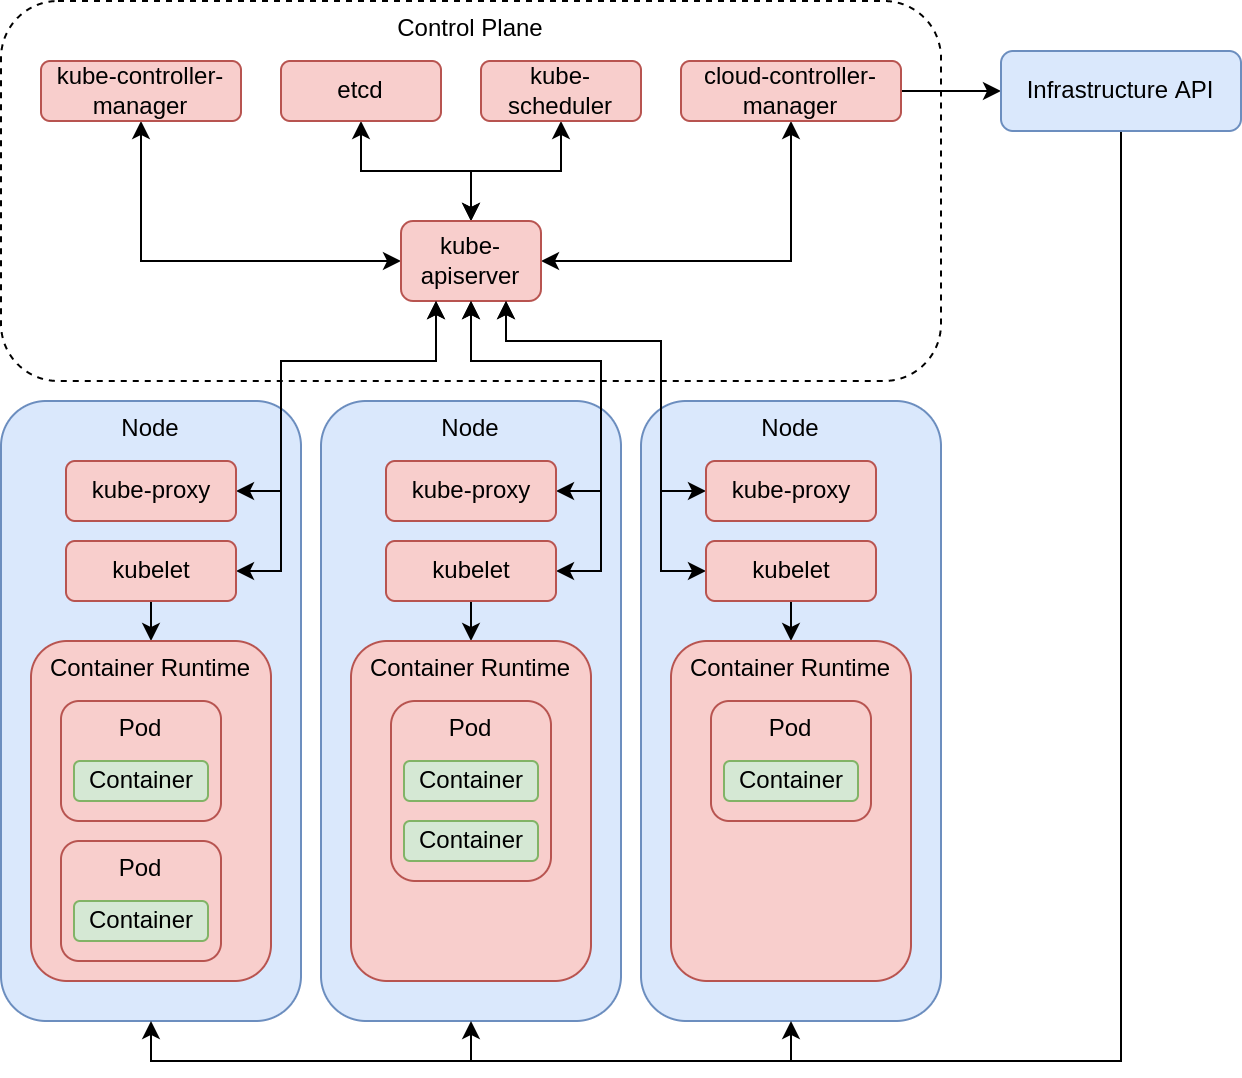
\includegraphics[width=\linewidth]{resources/kubernetes-overview.drawio.png}
  \caption{Overview of core Kubernetes components.}
  \label{fig:kubernetes-overview}
\end{figure}

We will first have look at an overview over the components of a Kubernetes
cluster. Figure \ref{fig:kubernetes-overview} can assist the reader in
understanding the relations between those components.

\begin{description}
  \item[Pods]
    A group of containers that share storage and network resources that models
    an application-specific logical host. The containers that make up a pod are
    always located on the same node and are scheduled in unison.

    In a broader sense, the pods are execution environments in which
    applications, in the form of containers, can be deployed and executed. As
    such, the pods are still part of the Platform layer, execution environments
    managed by an application orchestration service, and the containers
    are the applications of the Application layer.

  \item[Nodes]
    Nodes are machines running containerized applications. On each node run the
    following components: kubelet, container runtime, kube-proxy. The kubelet is
    an agent that is responsible for making sure that all containers of a pod
    are running, while the container runtime is the software that is actually
    responsible for running containers. The kube-proxy component allow the
    discovery of applications running inside the cluster and the exposure of
    those applications as services.

    These nodes correspond to compute resources of the Infrastructure layer. The
    components on those nods however are part of the Platform layer, as they
    implement specific functionalities needed in order to provide the services
    of the Platform layer.

  \item[Control Plane]
    A collection of components that manage nodes and pods inside the cluster,
    making global decisions about the cluster. This includes an API
    (kube-apiserver), a backing store (etcd) for all cluster data, and a
    scheduler (kube-scheduler) that assigns pods to nodes. Kubernetes adopts the
    concept of control loops, enabling the use of so-called controllers, which
    are non-terminating loops that watch the state of the cluster and make
    requests of changes when needed. While each of these controllers are
    logically separate processes, they are compiled into a single
    kube-controller-manager component. The management of Infrastructure layer
    resources is abstracted by the cloud-controller-manager which implements
    cloud specific resource management. All control plane components are also
    deployed in the Kubernetes cluster using pods.

    The components of the control plane implement specific behaviors, which
    together with the components on the nodes, provide the services of the
    Platform layer.
\end{description}

\subsubsection{Infrastructure Management and Security}

Kubernetes enables cloud providers to implement cloud specific infrastructure
management services by developing a cloud-controller-manager, Container Storage
Interface (CSI), and Container Network Interface (CNI), allowing tenants to
automatically scale their Kubernetes cluster depending on the current
utilization of infrastructure resources in order to be more cost-efficient.

The cloud-controller-manager typically consists of multiple components that
create and update load balancers, and manage the lifecycle of nodes.

CSI plugins are responsible for creating, updating, and destroying storage
resources in order to provide pods with persistent storage, referred to as
persistent volumes. Cloud providers often also provide storage encryption
services in conjunction with their storage resources. These encryption services
use keys provided by a KMS. While some cloud providers allow tenants to provide
their own KMS, the encryption service still needs plain text access to keys in
order to encrypt and decrypt data.

CNI plugins create, update, and destroy the underlying network resources of the
Kubernetes cluster and provide node-level, and pod-level communication. Some
CNIs also implement authentication and authorization that allow tenants to
enforce network policies in the cluster, and transparent encryption, protecting
confidential data traversing network resources.

\subsubsection{Application Orchestration}

The basic workflow of how Kubernetes deploys, configures, and starts a pod on a
node is as follows (see Figure \ref{fig:kubernetes-application-orchestration}).
Note that this description of the workflow is greatly simplified.

\begin{figure}[H]
  \centering
  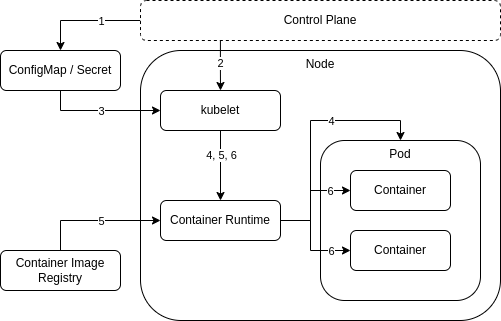
\includegraphics[width=0.7\linewidth]{resources/kubernetes-application-orchestration.drawio.png}
  \caption{Kubernetes' application deployment, configuration, and execution workflow.}
  \label{fig:kubernetes-application-orchestration}
\end{figure}

\begin{enumerate}
  \item Upon request of a tenant, the control plane creates ConfigMaps/Sects,
        which contain non-confidential/confidential configurations of an
        application.
  \item Upon request of a tenant, the control plane requests the kubelet of a
        node to create a pod and provides the kubelet with the specification of
        the pod. This specification includes container images,
        ConfigMaps/Secrets, storage configuration, and network configuration.
  \item Kubelet pulls specified ConfigMaps/Secrets onto the node.
  \item Kubelet calls the container runtime to create the pod, configure its
        storage and network, and provide the pod with the configurations of the
  \item Kubelet calls the container runtime to pull the specified container
        images.
  \item Kubelet calls the container runtime to create and start the application
        containers inside the pod using the pulled container images.
\end{enumerate}
